\documentclass{article}
% Change "article" to "report" to get rid of page number on title page
\usepackage{amsmath,amsfonts,amsthm,amssymb}
\usepackage{setspace}
\usepackage{Tabbing}
\usepackage{fancyhdr}
\usepackage{lastpage}
\usepackage{extramarks}
\usepackage{chngpage}
\usepackage{soul,color}
\usepackage{graphicx,float,wrapfig}
\usepackage{listings}

% In case you need to adjust margins:
\topmargin=-0.45in      %
\evensidemargin=0in     %
\oddsidemargin=0in      %
\textwidth=6.5in        %
\textheight=9.0in       %
\headsep=0.25in         %

% Homework Specific Information
\newcommand{\hmwkTitle}{Homework 1}
\newcommand{\hmwkDueDate}{Jan 29, 2013}
\newcommand{\hmwkClass}{Bayesian Statistical Methods}
\newcommand{\hmwkClassTime}{}
\newcommand{\hmwkClassInstructor}{}
\newcommand{\hmwkAuthorName}{Andrew Kurzawski}

% Setup the header and footer
\pagestyle{fancy}                                                       %
\lhead{\hmwkAuthorName}                                                 %
\chead{\hmwkClass\ (\hmwkClassInstructor\ \hmwkClassTime): \hmwkTitle}  %
\rhead{\firstxmark}                                                     %
\lfoot{\lastxmark}                                                      %
\cfoot{}                                                                %
\rfoot{Page\ \thepage\ of\ \pageref{LastPage}}                          %
\renewcommand\headrulewidth{0.4pt}                                      %
\renewcommand\footrulewidth{0.4pt}                                      %

% This is used to trace down (pin point) problems
% in latexing a document:
%\tracingall

%%%%%%%%%%%%%%%%%%%%%%%%%%%%%%%%%%%%%%%%%%%%%%%%%%%%%%%%%%%%%
% Some tools
\newcommand{\enterProblemHeader}[1]{\nobreak\extramarks{#1}{#1 continued on next page\ldots}\nobreak%
                                    \nobreak\extramarks{#1 (continued)}{#1 continued on next page\ldots}\nobreak}%
\newcommand{\exitProblemHeader}[1]{\nobreak\extramarks{#1 (continued)}{#1 continued on next page\ldots}\nobreak%
                                   \nobreak\extramarks{#1}{}\nobreak}%

\newlength{\labelLength}
\newcommand{\labelAnswer}[2]
  {\settowidth{\labelLength}{#1}%
   \addtolength{\labelLength}{0.25in}%
   \changetext{}{-\labelLength}{}{}{}%
   \noindent\fbox{\begin{minipage}[c]{\columnwidth}#2\end{minipage}}%
   \marginpar{\fbox{#1}}%

   % We put the blank space above in order to make sure this
   % \marginpar gets correctly placed.
   \changetext{}{+\labelLength}{}{}{}}%

\setcounter{secnumdepth}{0}
\newcommand{\homeworkProblemName}{}%
\newcounter{homeworkProblemCounter}%
\newenvironment{homeworkProblem}[1][Problem \arabic{homeworkProblemCounter}]%
  {\stepcounter{homeworkProblemCounter}%
   \renewcommand{\homeworkProblemName}{#1}%
   \section{\homeworkProblemName}%
   \enterProblemHeader{\homeworkProblemName}}%
  {\exitProblemHeader{\homeworkProblemName}}%

\newcommand{\problemAnswer}[1]
  {\noindent\fbox{\begin{minipage}[c]{\columnwidth}#1\end{minipage}}}%

\newcommand{\problemLAnswer}[1]
  {\labelAnswer{\homeworkProblemName}{#1}}

\newcommand{\homeworkSectionName}{}%
\newlength{\homeworkSectionLabelLength}{}%
\newenvironment{homeworkSection}[1]%
  {% We put this space here to make sure we're not connected to the above.
   % Otherwise the changetext can do funny things to the other margin

   \renewcommand{\homeworkSectionName}{#1}%
   \settowidth{\homeworkSectionLabelLength}{\homeworkSectionName}%
   \addtolength{\homeworkSectionLabelLength}{0.25in}%
   \changetext{}{-\homeworkSectionLabelLength}{}{}{}%
   \subsection{\homeworkSectionName}%
   \enterProblemHeader{\homeworkProblemName\ [\homeworkSectionName]}}%
  {\enterProblemHeader{\homeworkProblemName}%

   % We put the blank space above in order to make sure this margin
   % change doesn't happen too soon (otherwise \sectionAnswer's can
   % get ugly about their \marginpar placement.
   \changetext{}{+\homeworkSectionLabelLength}{}{}{}}%

\newcommand{\sectionAnswer}[1]
  {% We put this space here to make sure we're disconnected from the previous
   % passage

   \noindent\fbox{\begin{minipage}[c]{\columnwidth}#1\end{minipage}}%
   \enterProblemHeader{\homeworkProblemName}\exitProblemHeader{\homeworkProblemName}%
   \marginpar{\fbox{\homeworkSectionName}}%

   % We put the blank space above in order to make sure this
   % \marginpar gets correctly placed.
   }%

% Python Setup
\lstset{
  language=Python,
  showstringspaces=false,
  formfeed=\newpage,
  tabsize=4,
  commentstyle=\itshape,
  basicstyle=\ttfamily,
  morekeywords={models, lambda, forms}
}

% Uncomment lines and make changes to have a header
\newcommand{\code}[1]{ % change to [2]
  % \hrulefill
  % \subsection*{#1}
  \lstinputlisting{#1} % change to {#2}
  \vspace{2em}
}

%%%%%%%%%%%%%%%%%%%%%%%%%%%%%%%%%%%%%%%%%%%%%%%%%%%%%%%%%%%%%


%%%%%%%%%%%%%%%%%%%%%%%%%%%%%%%%%%%%%%%%%%%%%%%%%%%%%%%%%%%%%
% Make title
\title{\vspace{2in}\textmd{\textbf{\hmwkClass:\ \hmwkTitle}}\\\normalsize\vspace{0.1in}\small{Due\ on\ \hmwkDueDate}\\\vspace{0.1in}\large{\textit{\hmwkClassInstructor\ \hmwkClassTime}}\vspace{3in}}
\date{}
\author{\textbf{\hmwkAuthorName}}
%%%%%%%%%%%%%%%%%%%%%%%%%%%%%%%%%%%%%%%%%%%%%%%%%%%%%%%%%%%%%

\begin{document}
\begin{spacing}{1.1}
\maketitle
\newpage
% Uncomment the \tableofcontents and \newpage lines to get a Contents page
% Uncomment the \setcounter line as well if you do NOT want subsections
%       listed in Contents
%\setcounter{tocdepth}{1}
%\tableofcontents
%\newpage

% When problems are long, it may be desirable to put a \newpage or a
% \clearpage before each homeworkProblem environment

\clearpage
\begin{homeworkProblem}

I have decided to use the PyMC package to create a model and sample from the posterior distribution. The code is as follows:

\code{./Scripts/hw1_model.py}
\code{./Scripts/sampler.py}

The resulting posterior distributions are as follows:

\begin{figure}[ht]
\begin{center}
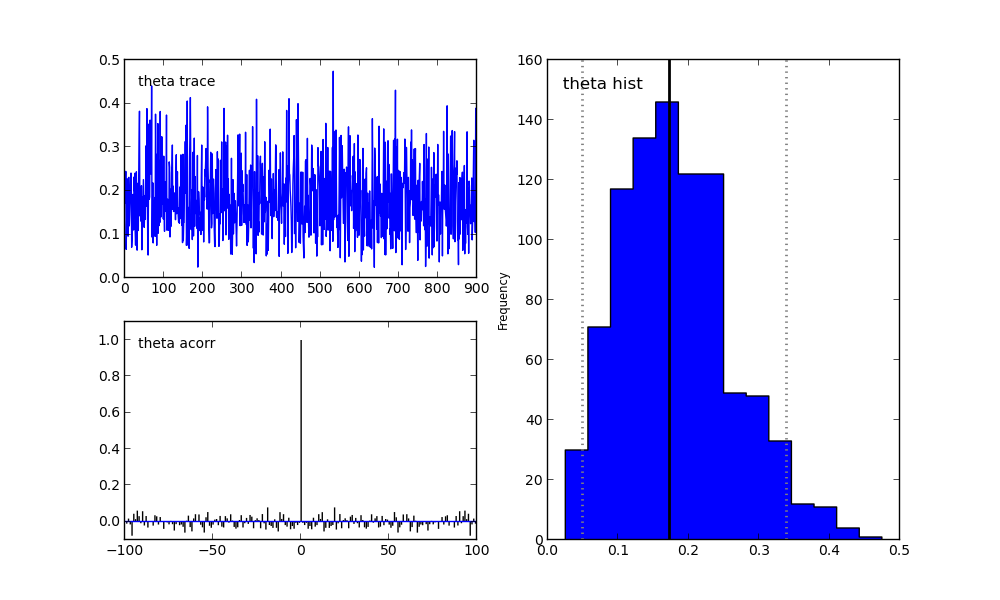
\includegraphics[height=3.0in]{./Figures/theta_1_1}
\end{center}
\caption{$\alpha = 1, \beta = 1$}
\label{fig:a1_b1}
\end{figure}

\begin{figure}[ht]
\begin{center}
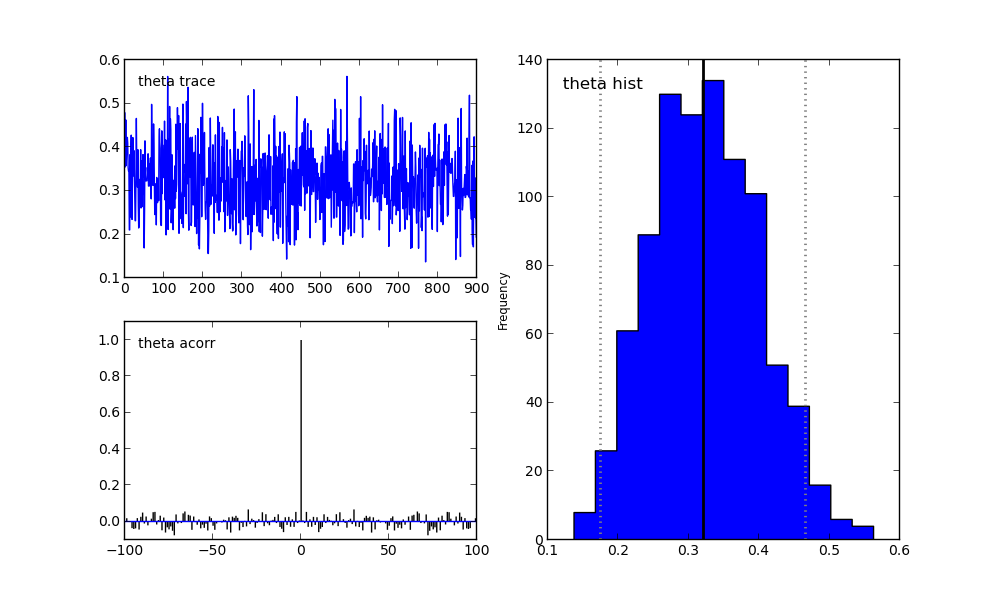
\includegraphics[height=3.0in]{./Figures/theta_10_10}
\end{center}
\caption{$\alpha = 10, \beta = 10$}
\label{fig:a10_b10}
\end{figure}

\begin{figure}[ht]
\begin{center}
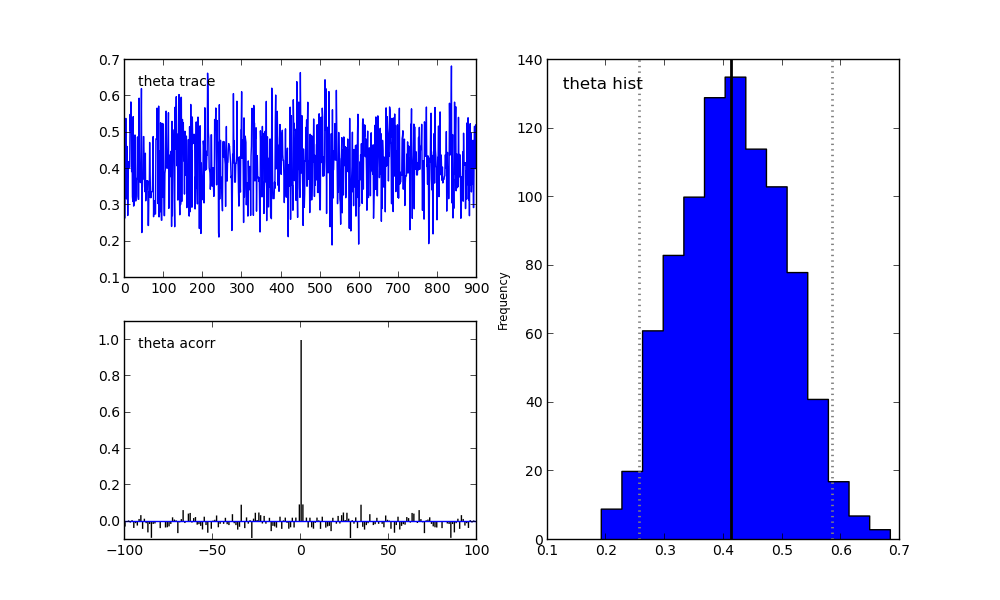
\includegraphics[height=3.0in]{./Figures/theta_10_1}
\end{center}
\caption{$\alpha = 10, \beta = 1$}
\label{fig:a10_b1}
\end{figure}

It is notable that the mode of the posterior given an uninformed prior (Fig.~\ref{fig:a1_b1}), is closest to 0.15 which corresponds to $Y=3$ after 20 trials. The influence of adding information to the prior in the form of the parameters $\alpha$ and $\beta$, can be seen in Fig.~\ref{fig:a10_b10} and~\ref{fig:a10_b1}. In these instances the priors did not have a uniform shape.

\end{homeworkProblem}

\clearpage
\begin{homeworkProblem}

For the case where a 20\% response rate has been observed, $\alpha$ and $\beta$ such that the mode of the prior distribution is 0.2. 

\begin{equation}
0.2 = \frac{\alpha - 1}{\alpha + \beta - 2}
\label{eq:beta_mode}
\end{equation}

Then, we could scale $\alpha$ and $\beta$ based on how much weight we wish to place on this previous observation.

\end{homeworkProblem}

\begin{homeworkProblem}

Derive Jeffreys' prior for the parameter in the Binomial model.

\begin{equation}
Y \sim Bin(n,\theta)
\label{eq:jeff_1}
\end{equation}

Where Jeffreys' prior is given as

\begin{equation}
J(\theta) = -E[\frac{\partial^2 log P(y|\theta)}{\partial \theta^2}]
\label{eq:jeff_2}
\end{equation}

and

\begin{equation}
P(y|\theta) = \dbinom{n}{y} \theta^y (1-\theta)^{n-y}
\label{eq:jeff_3}
\end{equation}

Then, we derive Jeffreys' prior taking the following steps.

\begin{equation}
logP(y|\theta) = log\dbinom{n}{y} + ylog\theta + (n-y) log (1-\theta)
\label{eq:jeff_4}
\end{equation}

\begin{equation}
\frac{\partial^2logP(y|\theta)}{\partial \theta^2} = -\frac{y}{\theta^2} - \frac{n-y}{(1-\theta)^2}
\label{eq:jeff_5}
\end{equation}

\begin{equation}
J(\theta) = -E[-\frac{y}{\theta^2} - \frac{n-y}{(1-\theta)^2}]
\label{eq:jeff_6}
\end{equation}

\begin{equation}
J(\theta) = \frac{n\theta}{\theta^2} + \frac{n-n\theta}{(1-\theta)^2}
\label{eq:jeff_7}
\end{equation}

Simplifying, we get:

\begin{problemAnswer}
{
\begin{equation}
J(\theta) = \frac{n}{\theta(1-\theta)}
\label{eq:jeff_8}
\end{equation}
}
\end{problemAnswer}

\end{homeworkProblem}

\clearpage
\begin{homeworkProblem}

\begin{equation}
P(\theta|y) \propto P(\theta)L(\theta|y)
\label{eq:4_1}
\end{equation}

For a Gamma distribution the probability density function is

\begin{equation}
P(\theta) = \frac{1}{\Gamma(a)b^a}\theta^{a-1}exp(\frac{-\theta}{b})
\label{eq:4_2}
\end{equation}

and the likelihood function $n$ independent Poisson responses is

\begin{equation}
L(\theta|y) = \frac{exp(-n\theta)\theta^{\Sigma y_i}}{\prod y_i!}
\label{eq:4_3}
\end{equation}

Combining Eqn.~\ref{eq:4_1},~\ref{eq:4_2} and~\ref{eq:4_3} while leaving out terms that do not depend on $\theta$.

\begin{equation}
P(\theta|y) \propto \theta^{a-1}exp \left(\frac{-\theta}{b} \right) exp\left(-n\theta \right)\theta^{\Sigma y_i}
\label{eq:4_4}
\end{equation}

Thus, the posterior distribution is a Gamma

\begin{problemAnswer}
{
\begin{equation}
P(\theta|y) \propto \theta^{a-1+\Sigma y_i}exp \left(-\theta (\frac{1}{b} + n) \right)
\label{eq:4_5}
\end{equation}

with parameters $a_o=a+\Sigma y_i$ and $b_o=\frac{1}{n+(1/b)}$.
}
\end{problemAnswer}

\end{homeworkProblem}

\begin{homeworkProblem}

\begin{equation}
P\left(\frac{1}{\sigma^2}|y\right) \propto P\left(\frac{1}{\sigma^2}\right)L\left(\frac{1}{\sigma^2}|y\right)
\label{eq:5_1}
\end{equation}

The likelihood of a Normal with a known mean is

\begin{equation}
L\left(\frac{1}{\sigma^2}|y\right) = \left(\frac{1}{2\pi \sigma^2}\right)^{\frac{n}{2}} exp \left[-\frac{1}{2\sigma^2} \sum (y_i-\mu)^2 \right]
\label{eq:5_2}
\end{equation}

Using Eqn.~\ref{eq:4_2} where $\theta$ is replaced by $\frac{1}{\sigma^2}$ and Eqn.~\ref{eq:5_2}, we can substitute into Eqn.~\ref{5_1}. Leaving out terms that do not depend on $\frac{1}{\sigma^2}$, we get that

\begin{equation}
P\left(\frac{1}{\sigma^2}|y\right) \propto \left(\frac{1}{\sigma^2}\right)^{a-1}exp\left(\frac{-1}{\sigma^2b}\right) \left(\frac{1}{2\pi \sigma^2}\right)^{\frac{n}{2}} exp \left[-\frac{1}{2\sigma^2} \sum (y_i-\mu)^2 \right]
\label{eq:5_3}
\end{equation}

Simplifying, the posterior becomes

\begin{problemAnswer}
{
\begin{equation}
P\left(\frac{1}{\sigma^2}|y\right) \propto \left(\frac{1}{\sigma^2}\right)^{a-1-\frac{n}{2}} exp \left[\frac{-1}{\sigma^2b}-\frac{1}{2\sigma^2} \sum (y_i-\mu)^2 \right]
\label{eq:5_4}
\end{equation}
}
\end{problemAnswer}

To bring in prior information on $\frac{1}{\sigma^2}$ to the Gamma distribution, we could take the mean, variance, and number of samples from a previous set of observations of $\frac{1}{\sigma^2}$ and calculate new values for $a$ and $b$ based on the form of Eqn.~\ref{eq:5_4}.

\end{homeworkProblem}

\end{spacing}
\end{document}

%%%%%%%%%%%%%%%%%%%%%%%%%%%%%%%%%%%%%%%%%%%%%%%%%%%%%%%%%%%%%

%----------------------------------------------------------------------%
% The following is copyright and licensing information for
% redistribution of this LaTeX source code; it also includes a liability
% statement. If this source code is not being redistributed to others,
% it may be omitted. It has no effect on the function of the above code.
%----------------------------------------------------------------------%
% Copyright (c) 2007, 2008, 2009, 2010, 2011 by Theodore P. Pavlic
%
% Unless otherwise expressly stated, this work is licensed under the
% Creative Commons Attribution-Noncommercial 3.0 United States License. To
% view a copy of this license, visit
% http://creativecommons.org/licenses/by-nc/3.0/us/ or send a letter to
% Creative Commons, 171 Second Street, Suite 300, San Francisco,
% California, 94105, USA.
%
% THE SOFTWARE IS PROVIDED "AS IS", WITHOUT WARRANTY OF ANY KIND, EXPRESS
% OR IMPLIED, INCLUDING BUT NOT LIMITED TO THE WARRANTIES OF
% MERCHANTABILITY, FITNESS FOR A PARTICULAR PURPOSE AND NONINFRINGEMENT.
% IN NO EVENT SHALL THE AUTHORS OR COPYRIGHT HOLDERS BE LIABLE FOR ANY
% CLAIM, DAMAGES OR OTHER LIABILITY, WHETHER IN AN ACTION OF CONTRACT,
% TORT OR OTHERWISE, ARISING FROM, OUT OF OR IN CONNECTION WITH THE
% SOFTWARE OR THE USE OR OTHER DEALINGS IN THE SOFTWARE.
%----------------------------------------------------------------------%